\section{Banken}
\begin{minipage}{0.5\linewidth}
	\begin{itemize}
		\item Banken erwirtschaften ihren Gewinn durch:
		\begin{itemize}
			\item Kreditvergabe mit geliehenem Geld (Zinsdifferenzgeschäft)
			\item Kommissionsgeschäft (Vermögensverwaltung, Investmentbanking)
			\item Eigenhandel
		\end{itemize}
		\item Finanzierung von Unternehmen:
		\begin{itemize}
			\item Finanzmärkte: direkte Finanzierung durch Aktien und Obligationen
			\item Banken: indirekte Finanzierung
		\end{itemize}
		Bei Beiden sind die Haushalte der Ursprung.
	\end{itemize}
\end{minipage}
\hspace{0.05\linewidth}
\begin{minipage}{0.4\linewidth}
	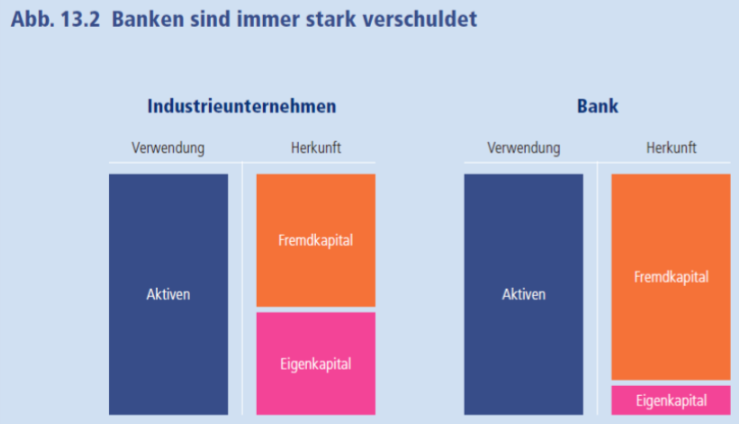
\includegraphics[width=\linewidth]{images/banken.png}
\end{minipage}
\begin{itemize}
	\item Banken als Finanzintermediäre (Zwischenliegende).
	Sie vermitteln das Kapital zwischen den Anlegern (den Haushalten) und den Kreditnehmern. Sie lösen dabei drei Probleme:
	\subitem 1. Transformation von Fristen (kurzfristige Perspektive der Kreditgeber vs. langfristige Perspektive der Kreditnehmer)
	\subitem 2. Bereitstellen von Informationen (asymmetrische Information zwischen uniformierten Kreditgebern und informierten Kapitalgebern)
	\subitem 3. Verteilung von Risiken (bei Kreditausfällen)
	\item keine Banken $\leftrightarrow$ keine Wirtschaft
\end{itemize}

\begin{multicols}{2}
	\subsection{Kreditvergabe als Bankgeschäft}
	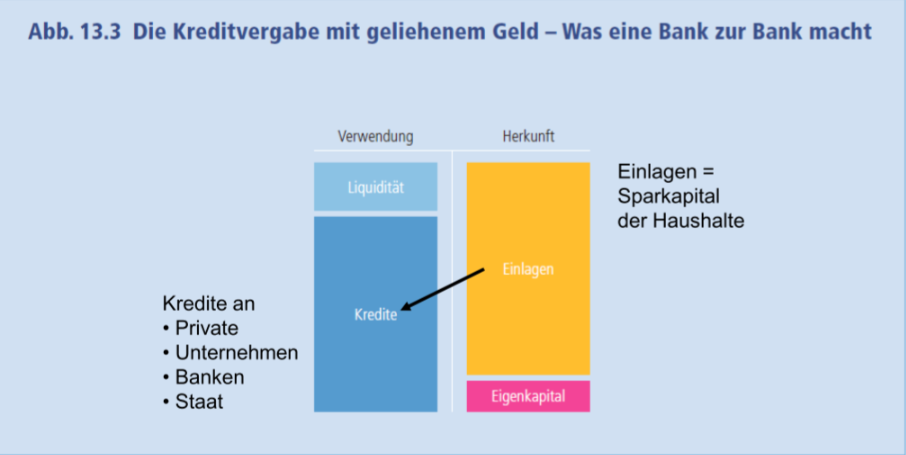
\includegraphics[width=\linewidth]{images/kreditvergabe.png}
	Liquidität kostet der Bank $\rightarrow$ auf ein Minimum eingeschränkt\\
	Banken gehen unter wenn entweder Eigenkapital oder Liquidität weg
	\columnbreak
	\subsection{Eigenhandel als Bankgeschäft}
	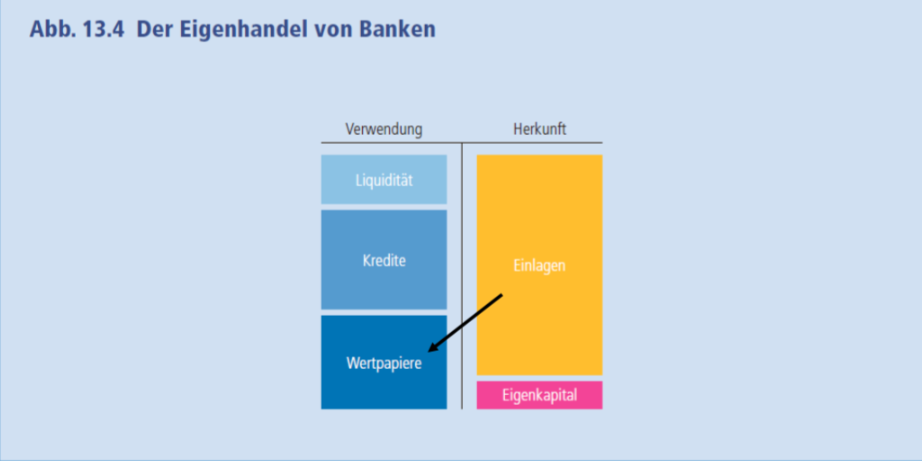
\includegraphics[width=\linewidth]{images/eigenhandel.png}
	Geht eine Bank konkurs, gehen auch die Unternehmen unter
\end{multicols}

\subsection{Risiken des Bankgeschäfts}
\begin{multicols}{2}
	\subsubsection{Liquiditätsrisiko (Passivseite)}
	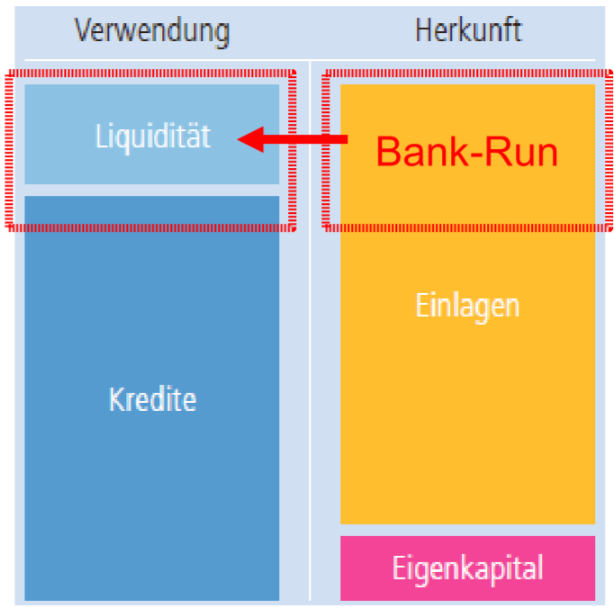
\includegraphics[width=0.5\linewidth]{images/liquiditaetsrisiko.png}\\
	Die Passivseite ist in der Regel kurzfristiger finanziert als die Aktivseite. Falls die Kreditgeber (Haushalte) massenweise ihr Geld zurückfordern $\rightarrow$ Bank-Run.
	\vfill\null
	\columnbreak
	\subsubsection{Solvenzrisiken (Aktivseite)}
	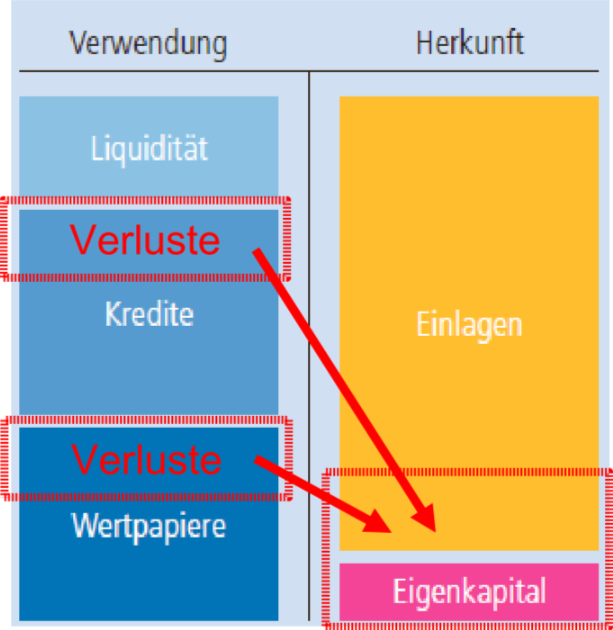
\includegraphics[width=0.5\linewidth]{images/solvenzrisiken.png}\\
	Wenn die Bank auf der Aktivseite (verliehene Kredite) Verluste erleidet. Zum Beispiel bei Kreditausfällen oder Wertverminderung der Wertpapiere. Diese Verluste müssen durch das Eigenkapital gedeckt werden können.
\end{multicols}

\subsection{Bankenregulierung}
Die Banken gehören zu den stärksten regulierten Branchen. Als Schutz für die Kunden und für die Stabilität des Finanzsystems.\\
\begin{minipage}{0.6\linewidth}
	\begin{itemize}
		\item \textbf{Mikroprudentielle Regulierung (Stabilität einzelner Banken):}\\
		Aufgabe der FINMA $\rightarrow$ kontrolliert Eigenkapital und Liquiditätsaustattung.
		\item \textbf{Makroprudentielle Regulierung (Stabilität des gesamten Bankensystems):}\\
		Aufgabe der SNB $\rightarrow$ setzt dabei auf Beobachtung und Entwicklung der Finanzmärkte (Prävention), wirkt bei den rechtlichen Rahmenbedingung mit und bietet eine Kurzfristige Vorsorge im Krisenfall
	\end{itemize}
\vfill\null
\end{minipage}%
\hspace{0.05\linewidth}
\begin{minipage}{0.3\linewidth}
	\includegraphics[width=0.8\linewidth]{images/banken2.jpg}
\end{minipage}

\subsubsection{Vorschriften}
\begin{itemize}
	\item Eigenkapitalquote (Passivseite)
	\subitem Basel II (8\%) und Basel III (13\%)
	\item Liquiditätsvorschriften
	\begin{description}
		\item[Obligatorische Einlageversicherung:] Dies verhindert Bank-Runs, da der Kunde weiss, dass er sein Geld (bis zu einer definierten Obergrenze) trotz Liquiditätsproblemen der Bank zurück erhält.
		\item[Liquiditätsvorgaben:] Die Bank muss einen bestimmten Prozentsatz der Aktiven als flüssige Mittel halten. Dies ist für die Banken teuer (sie hat keine Erträge aus diesen Mitteln). Deshalb versuchen sich die Banken vor allem auf dem Geldmarkt bei anderen Banken zu finanzieren, da dieses Kapital in der Regel günstiger ist als das zur Verfügung gestellte Kapital der Haushalte.
		\begin{itemize}
			\item{\makebox[5cm]{Kredite an Zentralregierungen\hfill}} 20\%
			\item{\makebox[5cm]{Wohnbauhypotheken\hfill}} 35\%
			\item{\makebox[5cm]{Interbankenkredite\hfill}} 20\%
			\item{\makebox[5cm]{Gewerbliche Hypotheken\hfill}} 100\%
			\item{\makebox[5cm]{Privatkundenkredite\hfill}} 75\%
		\end{itemize}
	\end{description}
	\item Makroprudentielle Vorschriften zur Konkursabwicklung
\end{itemize}

\subsubsection{Too Big to Fail}
Die gegenseitige kurzfristige Finanzierung von Banken in Form des Interbanken-Geschäfts (zwecks Liquiditätssicherung, aber teilweise auch für den Eigenhandel) führt zu einer starken Verflechtung des Bankensektors. Kommt es zu einem Bank-Run bei einer grossen Bank, können auch andere kreditgebende Banken unter Druck geraten. In einem solchen Fall müssen Zentralbanken bzw. Regierungen die insolventen Banken retten. Ein Scheitern dieser Banken würde unabsehbare Folgen für die Volkswirtschaft mit sich ziehen. Dies schafft eine unhaltbare Situation: die Banken werden ihre Risiken maximieren. Die Gewinne werden damit privatisiert, während die Allgemeinheit für die allfälligen Verluste aufkommen muss (entspricht faktisch einer $"$Staatsgarantie$"$).\\
\textbf{Lösungsansätze dazu}\\
\begin{itemize}
	\item 1. Insolvenzverhinderung durch höhere Eigenkapitalanforderungen, welche konjunkturzyklisch schwanken und damit als automatische Stabilisatoren wirken (bei Rezession tiefere, bei Hochkonjunktur höhere Vorschriften)
	\item 2. Verfahren zur Konkursabwicklung beschrieben in Form eines $"$living will$"$ (funktionsfähige Geschäftsbereiche rasch abspalten)
\end{itemize}
\begin{centering}
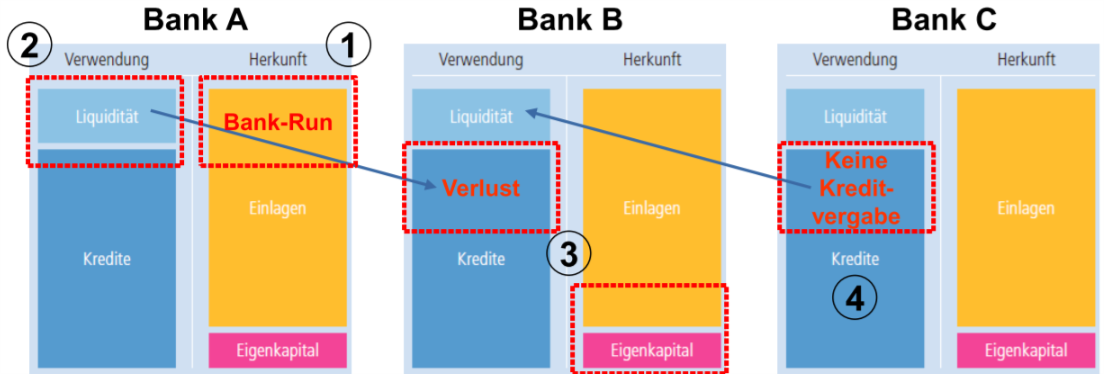
\includegraphics[width=0.9\linewidth]{images/toobig.png}
\end{centering}

\clearpage
\pagebreak
